\documentclass[a4paper,10pt]{article}

\usepackage{graphicx}
\usepackage{url}
\usepackage{times}
\usepackage{color}
\usepackage{floatpag}

\newcommand{\mysection}[1]{\section{#1}\label{#1}}
\newcommand{\mysubsection}[1]{\subsection{#1}\label{#1}}
\newcommand{\mysubsubsection}[1]{\subsubsection{#1}\label{#1}}
\newcommand{\remark}[1]{[\emph{#1}]}

\begin{document}

\title{The Ibis GMI (Group Method Invocation) Programmers Manual}

\author{The Ibis Group}

\maketitle

\section{Introduction}

For many parallel and distributed applications, the simple synchronous
unicast communication model (one-to-one communication with a reply)
offered by RMI is inadequate.  Applications often require more
different, more complex forms of communication, such as asynchronous
unicast (one-to-one communication without a reply), broadcast
(one-to-all communication), multicast (one-to-many communication), or
data reduction operations (where data must be collected from multiple
machines).  Although these alternative forms of communication can be
implemented using RMI, this is often complex and inefficient. For
example, a simple way to implement multicast is to perform multiple
RMI calls, one after the other. Unfortunately, this is very
inefficient, since each RMI must wait until the previous RMI has
finished completely, including waiting for the (unused) result to be
returned. More efficient implementations use threads to perform
multiple RMIs simultaneously or create distributed multicast trees
which use multiple machines to forward calls. These implementations
are complex, however, and often suffer from performance problems
caused by the synchronous nature of RMI.  In Ibis, we offer a new
programming model called GMI (Group Method Invocation). GMI is an
extension of RMI designed to be flexible enough to express the complex
forms of communication needed by many parallel
applications. Nevertheless, GMI is as easy to use as RMI, hiding the
complex details of the communication in its implementation. The
flexible model of GMI also allows its implementation to use efficient
communication algorithms for multicast, data reduction, etc. The GMI
model will be explained in detail below.


\mysection{The GMI model}

The GMI model generalizes the RMI model in three ways. First, it
introduces the notion of a 'group', a set of objects which all
implement the same interface. The objects in a group may be
distributed over a number of JVMs. A group can be addressed using a
single 'group reference'. An example is shown in Figure~\ref{gmi-fig}, where an
application thread uses a single group reference to address a group of
two objects (on different JVMs).

\begin{figure}[t]
\begin{center}
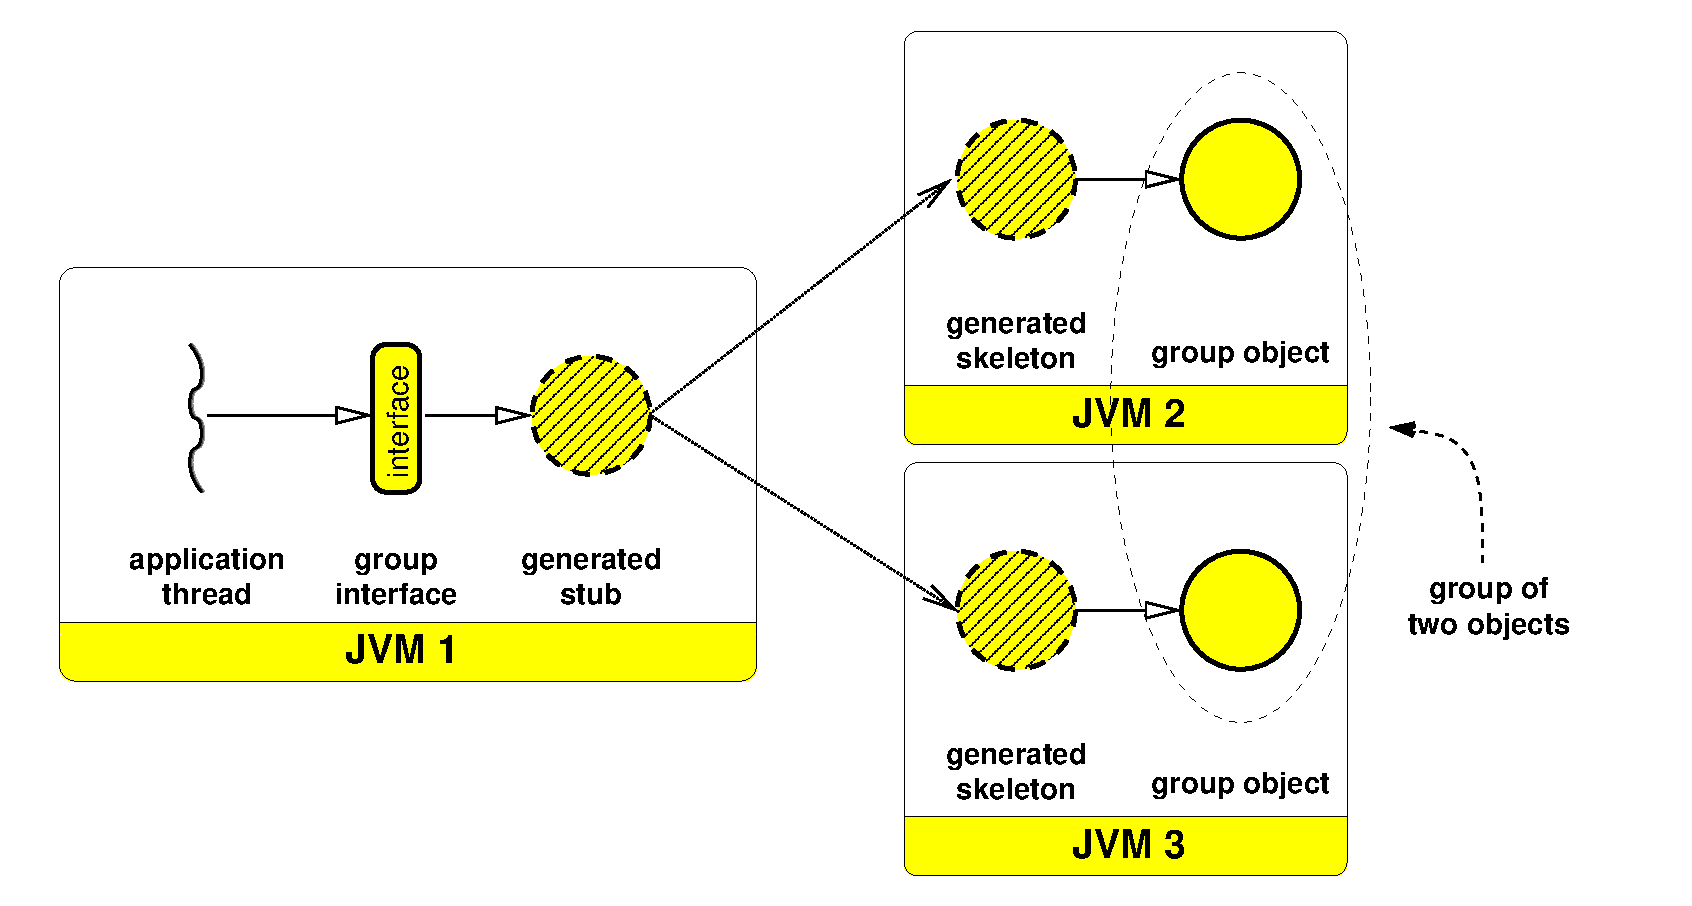
\includegraphics[width=0.7\textwidth]{gmi-abstract.eps}
\end{center}
\caption{A group invocation with GMI.}
\label{gmi-fig}
\end{figure}

Like RMI, GMI uses compiler generated stub and skeleton objects which
implement the necessary communication code. The application programmer
does not have to write any communication code. Unlike RMI, however,
GMI does not only generate code for synchronous unicast
communication. Instead, many different types of communication code are
generated, both for sending of method invocations and for returning of
results. This is the second generalization introduced by GMI.
Finally, through a simple API, the programmer can configure at run
time which type of communication should be used to handle each
individual method of a group reference. This API will be explained in
more detail in the next section. Different ways of forwarding the
invocation and handling the results can be combined, giving a rich
variety of communication mechanisms. By configuring the methods at run
time, the communication behavior of the application can easily be
adapted to changing requirements.

The following types of method invocation forwarding are currently
supported by GMI:
\begin{itemize}
\item{single invocation:}
The method invocation is
forwarded to a single object of the group, identified via a rank.
\item{group invocation:}
The invocation is forwarded to every object in the
group.
\item{personalized group invocation:}
The invocation is forwarded to
every object in the group, while the parameters are personalized for
each destination using a user-defined method.
\item{combined invocation:}
Multiple application threads (possibly on multiple JVMs) invoke the
same method on the same group. These invocations are combined into a
single invocation using a user-defined method. This single invocation
is forwarded to the group using one of the three other forwarding
schemes.
\end{itemize}

The following types of method result handling are currently supported
by GMI:
\begin{itemize}
\item{discard results:}
No results are returned at all (including
exceptions).
\item{return one result:}
A single result is returned,
preselected via a rank if neccesary.
\item{forward results:}
All results are
returned, but they are forwarded to a user-defined object rather than
being returned to the invoking thread.
\item{combine results:}
Combine all
results into a single one using a user-defined method. The combined
result is returned to the invoker.
\item{personalize result:}
A result
produced by one of the other result handling schemes is personalized
using a user-defined method before being returned to each of the
invokers (this is useful when a combined invocation is used).  The
four different forwarding schemes and five different result handling
schemes can be combined orthogonally, resulting in a wide variety of
useful communication patterns.  
\end{itemize}

\mysection{Hello world in GMI}

We will now show a
step by step example of how a GMI application can be written. The
first step is to create an interface which will define the methods
which can be invoked on the group of objects. Like in RMI, we use a
special 'marker interface' to 'mark' group interfaces. Any interface
extending ibis.gmi.GroupInterface will be recognized by the Ibis
compiler as being a group interface. The Ibis compiler will then
generate a stub object which contains the necessary communication
code.

{\small
\begin{quote}
\begin{verbatim}
interface Example extends ibis.gmi.GroupInterface {
   public void put(String message);
   public String get();
}
\end{verbatim}
\end{quote}
}
\noindent

In the example above, the 'Example' interface is turned into a group
interface by extending ibis.gmi.GroupInterface. It defines just two
methods, put, which can be used to store a string, and get which can
be used to retrieve a stored string.  After creating the group
interface, an implementation of this interface is be created. This
implementation object must implement the Example interface, and extend
the ibis.gmi.GroupMember object, which contains some basic
functionality needed to be part of a group (this is similar to the
UnicastRemoteObject used in RMI).

\begin{figure}[t!]
{\small
\begin{verbatim}
import ibis.gmi.GroupMember;

class Implementation extends GroupMember implements Example {

   private String message = null;

   public synchronized void put(String message) {
      this.message = message;
      notify();
   }
   
   public synchronized String get() { 
      while (message == null) { 
         wait();
      }       
      return message;
   } 
}
\end{verbatim}
}
\caption{Implementing a group object with GMI.}
\label{gmi-1}
\end{figure}

In this implementation, shown in Figure~\ref{gmi-1}, the put method stores the
string it receives in the object, from where it can be retrieved using
the get method. The standard synchronization primitives synchronized,
wait, and notify are used to prevent the get from returning before the
string is available.  Next, we will create an simple example
application, BroadcastExample, which will use the group object. The
source code is shown in Figure~\ref{gmi-2}. This application is parallel; it is
designed to be started simultaneously on multiple JVMs.

\begin{figure}[t!]
{\small
\begin{verbatim}
import ibis.gmi.*;

class BroadcastExample {

   public static void main(String[] args) {
      int size = Group.size();
      int rank = Group.rank();

      if (rank == 0) {
         // JVM 0 creates a new group. 
         Group.create("ExampleGroup", Example.class, size);
      } 

      // All JVMs create an implementation object.
      Implementation impl = new Implementation();
   
      // And join the group
      Group.join("ExampleGroup", impl);

      if (rank == size-1) { 
         // The last JVM retrieves a group reference
         Example group = (Example) Group.lookup("ExampleGroup");

         // Then configures 'put' to be forwarded to the whole group
         GroupMethod m = Group.findMethod(group, "void put(java.lang.String)");
         m.configure(new GroupInvocation(), new DiscardReply());

         // Now invoke a method on the group
         group.put("Hello world!");
      } 

      // All JVMs can now retrieve the data using a local(!) call
      String message = impl.get();        
      System.out.println(message);

      // Done   
      Group.exit();
   }
} 
\end{verbatim}
}
\caption{An example GMI application that uses a group object.}
\label{gmi-2}
\end{figure}

The main method of the application starts by invoking Group.size and
Group.rank, two utility methods of GMI which can be used to find out
how many JVMs are available (size), and what number is assigned to the
current JVM (rank).  The JVM with rank 0 then creates a new group
using Group.create. This group will have the name ExampleGroup, use a
group interface of the type Example and will contain 'size'
objects. Each JVM then creates it's own Implementation object, and
adds it to the group using the Group.join method. Group.join will
block until all 'size' objects have been added to the group.  The last
JVM (with rank 'size-1') then retrieves a group reference using
Group.lookup. This method will return a stub generated by the Ibis
compiler. This stub contains the communication code necessary to
communicate with the objects in the group. Because the stub implements
the Example interface, normal invocations of the put and get methods
can be used and no communication code needs to be written by the
programmer. But before the methods can be invoked, the group stub must
first be configured.  All methods in a group stub can be configured
separately. In this example we will only use the put method. To
configure put, we first perform a lookup of the method using
Group.findMethod. A GroupMethod object will be returned, which
represents the put method of the stub.  Using the configure method in
this GroupMethod object, it can be specified how the invocations of
the put method should be handled. For this purpose the configure
method takes two parameters, one describing how the invocation must be
forwarded to the group, and one describing how the replies should be
returned. In the example application we use GroupInvocation and
DiscardReply, which indicates that invocations of put will be
forwarded to all objects in the group, and that no replies will be
returned.  After the configuration is completed, the last JVM invokes
the put method. The method invocation is then forwarded to all object
in the group. All JVMs then retrieve their local copy of the string by
directly invoking the get method on their implementation objects.

\section{Further Reading}

The Javadoc included in the \texttt{javadoc} directory has detailed
information on all classes and their methods.

The Ibis web page \url{http://www.cs.vu.nl/ibis} lists all
the documentation and software available for Ibis, including papers, and
slides of presentations.

For detailed information on running a GMI application see the
User's Manual, available in the docs directory of the Ibis GMI
distribution.

\end{document}
